%!TEX encoding = UTF-8 Unicode
%!TEX root = ../lect-w09.tex

%%%


%\begin{Slide}{TODO: Begrepp att förklara}
%  Tänk igenom ordningen:
%  \begin{itemize}
%    \item OO, arv, supertyp, subtyp, bastyp, polymorfism, ... 
%  \end{itemize}
%\end{Slide}


\Subsection{Vad är arv?}

\begin{Slide}{Vad är arv?}

\begin{minipage}{0.4\textwidth}
\raggedright Med arv kan man beskriva relationen \\
$X$ \Emph{är en} $Y$

\end{minipage}
\begin{minipage}{0.4\textwidth}
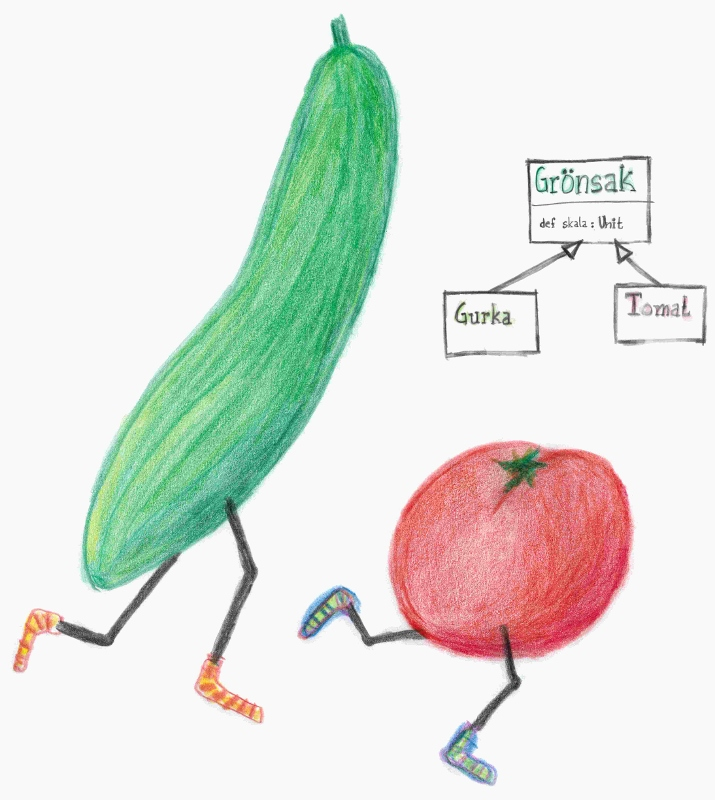
\includegraphics[width=1.5\textwidth]{../img/gurka-tomat-715x800}
\end{minipage} 
\end{Slide}


\begin{Slide}{Varför behövs arv?}
\begin{itemize}
\item Man kan använda arv för att dela upp kod i: 
\begin{itemize}
\item \Emph{generella} (gemensamma) delar och 
\item \Emph{specifika} (specialanpassade) delar.
\end{itemize}

\item Man kan åstadkomma \Emph{kontrollerad flexibilitet}: 
\begin{itemize}
\item Klientkod kan \Emph{utvidga} \Eng{extend} ett givet API med egna specifika tillägg.
\end{itemize}

\item Man kan använda arv för att deklarera en gemensam \Emph{bastyp} så att generiska samlingar kan ges en mer specifik elementtyp. 
\begin{itemize}
\item Det räcker att man vet bastypen för att kunna anropa gemensamma metoder på alla element i samlingen.
\end{itemize}
\end{itemize}
\end{Slide}


\begin{Slide}{Behovet av gemensam bastyp}\SlideFontSmall
\begin{REPL}
scala> class Gurka(val vikt: Int)

scala> class Tomat(val vikt: Int)

scala> val gurkor = Vector(new Gurka(200), new Gurka(300))
gurkor: scala.collection.immutable.Vector[Gurka] = 
  Vector(Gurka@60856961, Gurka@2fd953a6)
  
scala> gurkor.map(_.vikt)
res0: scala.collection.immutable.Vector[Int] = Vector(200, 300)

scala> val grönsaker = Vector(new Gurka(200), new Tomat(42))
grönsaker: scala.collection.immutable.Vector[Object] = 
  Vector(Gurka@669253b7, Tomat@5305c37d)

scala> grönsaker.map(_.vikt)
<console>:15: error: value vikt is not a member of Object
       grönsaker.map(_.vikt)
\end{REPL}
Hur ordna en mer specifik typ än \code{Vector[Object]}? \pause$\rightarrow$ Skapa en \Emph{bastyp}!
\end{Slide}




\begin{Slide}{Skapa en gemensam bastyp}
Typen \textit{\textbf{\texttt{Grönsak}}} är en \Emph{bastyp} i nedan arvshierarki:

\vspace{1em}
\begin{center}
\newcommand{\TextBox}[1]{\raisebox{0pt}[1em][0.5em]{#1}}
\tikzstyle{umlclass}=[rectangle, draw=black,  thick, anchor=north, text width=2cm, rectangle split, rectangle split parts = 3]
\begin{tikzpicture}[inner sep=0.5em]
\node [umlclass, rectangle split parts = 1, xshift=0cm] (BaseType)  {
            \textit{\textbf{\centerline{\TextBox{\code{Grönsak}}}}}
            %\nodepart[]{second}\TextBox{\code{val vikt: Int}}
        };
        
\node [umlclass, rectangle split parts = 1]  at (2cm,-2cm) (SubType1) {
            \textbf{\centerline{\TextBox{\code{Gurka}}}}
            %\nodepart[]{second} \TextBox{~}
        };  
                
\node [umlclass, rectangle split parts = 1] at (-2cm,-2cm) (SubType2)  {
            \textbf{\centerline{\TextBox{\code{Tomat}}}}
            %\nodepart[]{second} \TextBox{talk(): void}
        };        
\draw[umlarrow] (SubType1.north) -- ++(0,0.5) -| (BaseType.south);    
\draw[umlarrow] (SubType2.north) -- ++(0,0.5) -| (BaseType.south);            
\end{tikzpicture}

\pause
\vspace{2em} Pilen ~ \tikz\draw[umlarrow] (0,0) -- (0,0.5); ~ betecknar \Emph{arv} och utläses ''\Alert{är en}''

\pause
{\vspace{1em}\SlideFontSmall Typerna \code{Tomat} och \code{Gurka} är \Emph{subtyper} till den \Emph{abstrakta} typen \code{Grönsak}.}
\end{center}
\end{Slide}







\begin{Slide}{Skapa en gemensam bastyp med \texttt{trait} och \texttt{extends}}\SlideFontSmall
Med \code{trait Grönsak} kan klasserna \code{Gurka} och \code{Tomat} få en gemensam \Emph{bastyp} genom att båda \Emph{subtyperna} gör \code{extends Grönsak}:
\begin{REPL}
scala> trait Grönsak

scala> class Gurka(val vikt: Int) extends Grönsak

scala> class Tomat(val vikt: Int) extends Grönsak

scala> val grönsaker = Vector(new Gurka(200), new Tomat(42))
grönsaker: scala.collection.immutable.Vector[Grönsak] = 
  Vector(Gurka@3dc4ed6f, Tomat@2823b7c5)


\end{REPL}
\pause
Men det är fortfarande inte som vi vill ha det:
\begin{REPLnonum}
scala> grönsaker.map(_.vikt)
<console>:15: error: value vikt is not a member of Grönsak
       grönsaker.map(_.vikt)
\end{REPLnonum}
\end{Slide}



\begin{Slide}{En gemensam bastyp med gemensamma delar}\SlideFontSmall
Placera gemensamma medlemmar i bastypen:

\vspace{1em}
\begin{center}
\newcommand{\TextBox}[1]{\raisebox{0pt}[1em][0.5em]{#1}}
\tikzstyle{umlclass}=[rectangle, draw=black,  thick, anchor=north, text width=3cm, rectangle split, rectangle split parts = 3]
\begin{tikzpicture}[inner sep=0.5em]
\node [umlclass, rectangle split parts = 2, xshift=0cm] (BaseType)  {
            \textit{\textbf{\centerline{\TextBox{\code{Grönsak}}}}}
            \nodepart[]{second}\TextBox{\code{val vikt: Int}}
        };
        
\node [umlclass, rectangle split parts = 1]  at (2cm,-3cm) (SubType1) {
            \textbf{\centerline{\TextBox{\code{Gurka}}}}
            %\nodepart[]{second} \TextBox{~}
        };  
                
\node [umlclass, rectangle split parts = 1] at (-2cm,-3cm) (SubType2)  {
            \textbf{\centerline{\TextBox{\code{Tomat}}}}
            %\nodepart[]{second} \TextBox{talk(): void}
        };        
\draw[umlarrow] (SubType1.north) -- ++(0,0.5) -| (BaseType.south);    
\draw[umlarrow] (SubType2.north) -- ++(0,0.5) -| (BaseType.south);            
\end{tikzpicture}
\end{center}
\vspace{2em} 
\begin{itemize}
\item Alla grönsaker har attributet \code{val vikt}. 
\item Det specifika värdet på vikten definieras \Alert{inte} i bastypen. 
\item Medlemen \code{vikt} kallas  \Emph{abstrakt} eftersom den \Alert{saknar implementation}.
\end{itemize}
\end{Slide}





\begin{Slide}{Placera gemensamma delar i bastypen}

Vi inkluderar det gemensamma attributet \code{val vikt} som en \Emph{abstrakt medlem} i bastypen:

\begin{Code}
trait Grönsak { val vikt: Int }

class Gurka(val vikt: Int) extends Grönsak

class Tomat(val vikt: Int) extends Grönsak
\end{Code}
Nu vet kompilatorn att alla grönsaker har en vikt: 
\begin{REPL}
scala> val grönsaker = Vector(new Gurka(200), new Tomat(42))
grönsaker: scala.collection.immutable.Vector[Grönsak] = 
  Vector(Gurka@3dc4ed6f, Tomat@2823b7c5)

scala> grönsaker.map(_.vikt)
res0: scala.collection.immutable.Vector[Int] = Vector(200, 42)
\end{REPL}

\end{Slide}





\begin{Slide}{Scalas typhierarki och typen \texttt{Object}}
Den översta delen av typhierarkin i Scala: 
\vspace{1em}
\begin{center}
\newcommand{\TextBox}[1]{\raisebox{0pt}[1em][0.5em]{#1}}
\tikzstyle{umlclass}=[rectangle, draw=black,  thick, anchor=north, text width=2.5cm, rectangle split, rectangle split parts = 3]
\begin{tikzpicture}[inner sep=0.5em]
\node [umlclass, rectangle split parts = 1, xshift=0cm] (BaseType)  {
            \textit{\textbf{\centerline{\TextBox{\code{Any}}}}}
            %\nodepart[]{second}\TextBox{\code{def toString: String}}
        };
        
\node [umlclass, rectangle split parts = 1]  at (2cm,-2cm) (SubType1) {
            \textit{\textbf{\centerline{\TextBox{\code{AnyRef}}}}}
            %\nodepart[]{second} \TextBox{~}
        };  
                
\node [umlclass, rectangle split parts = 1] at (-2cm,-2cm) (SubType2)  {
            \textit{\textbf{\centerline{\TextBox{\code{AnyVal}}}}}
            %\nodepart[]{second} \TextBox{talk(): void}
        };        
\draw[umlarrow] (SubType1.north) -- ++(0,0.5) -| (BaseType.south);    
\draw[umlarrow] (SubType2.north) -- ++(0,0.5) -| (BaseType.south);            
\end{tikzpicture}
\end{center}
\begin{itemize}\SlideFontSmall
\item De numeriska typerna \code{Int}, \code{Double}, etc är subtyper till \Emph{\code{AnyVal}} och kallas \Emph{värdetyper} och lagras på ett speciellt, effektivt sätt i minnet.  
\item Alla dina egna klasser är subtyper till \Emph{\texttt{AnyRef}} och kallas \Emph{referenstyper} och kräver (direkt eller indirekt) konstruktion med \code{new}.
\item \texttt{AnyRef} motsvaras av \Alert{\code{java.lang.Object}} i JVM.
\end{itemize}
\end{Slide}



\begin{Slide}{Implicita supertyper till dina egna klasser}
Alla dina egna typer ingår underförstått i Scalas typhierarki:

\vspace{1em}
\begin{center}
\newcommand{\TextBox}[1]{\raisebox{0pt}[1em][0.5em]{#1}}
\tikzstyle{umlclass}=[rectangle, draw=black,  thick, anchor=north, text width=2cm, rectangle split, rectangle split parts = 3]
\begin{tikzpicture}[inner sep=0.5em, scale=0.8, every node/.style={scale=0.8}]
\node [umlclass, rectangle split parts = 1, xshift=0cm] at (0,-0.3cm)(BaseType)  {
            \textit{\textbf{\centerline{\TextBox{\code{Any}}}}}
            %\nodepart[]{second}\TextBox{\code{def toString: String}}
        };
        
\node [umlclass, rectangle split parts = 1]  at (2cm,-2cm) (SubType1) {
            \textit{\textbf{\centerline{\TextBox{\code{AnyRef}}}}}
            %\nodepart[]{second} \TextBox{~}
        };  
                
\node [umlclass, rectangle split parts = 1] at (-2cm,-2cm) (SubType2)  {
            \textit{\textbf{\centerline{\TextBox{\code{AnyVal}}}}}
            %\nodepart[]{second} \TextBox{talk(): void}
        };        
        
        
\node [umlclass, rectangle split parts = 1] at (2cm,-3.5cm) (SubSubType)  {
            \textit{\textbf{\centerline{\TextBox{\code{Grönsak}}}}}
            %\nodepart[]{second} \TextBox{talk(): void}
        }; 
        
\node [umlclass, rectangle split parts = 1] at (3.5cm,-5.25cm) (SubSubSubType1)  {
            \textbf{\centerline{\TextBox{\code{Gurka}}}}
            %\nodepart[]{second} \TextBox{talk(): void}
        }; 
                
\node [umlclass, rectangle split parts = 1] at (0.5cm,-5.25cm) (SubSubSubType2)  {
            \textbf{\centerline{\TextBox{\code{Tomat}}}}
            %\nodepart[]{second} \TextBox{talk(): void}
        }; 

                
\draw[umlarrow] (SubType1.north) -- ++(0,0.3) -| (BaseType.south);    
\draw[umlarrow] (SubType2.north) -- ++(0,0.3) -| (BaseType.south);   
\draw[umlarrow] (SubSubType.north) -- (SubType1.south);    
\draw[umlarrow] (SubSubSubType1.north) -- ++(0,0.3) -| (SubSubType.south);    
\draw[umlarrow] (SubSubSubType2.north) -- ++(0,0.3) -| (SubSubType.south);                   
\end{tikzpicture}
\end{center}
\end{Slide}


\begin{Slide}{Vad är en trait?}
\begin{itemize}
\item \Alert{Trait} betyder \Emph{egenskap} på engelska.

\item En trait liknar en klass, \Alert{men} speciella regler gäller:  

\begin{itemize}

\item den \Emph{kan} innehålla delar som \Emph{saknar implementation}

\item den \Emph{kan mixas} med flera andra traits så att olika koddelar kan återanvändas på flexibla sätt. 

\item den \Alert{kan inte} instansieras direkt som den är.

\item den \Alert{kan inte} ha klassparametrar eller konstruktorer.
\end{itemize}

\pause
\item {\SlideFontSmall Jämförelse med Java:} 
\begin{itemize}\SlideFontTiny
\item En Scala-trait liknar det som i Java kallas \jcode{interface}, men man kan göra mer med Scala-traits: färre begränsningar, fler abstraktionsmöjligheter.

\item En Scala-trait med enbart abstrakta medlemmar kompileras till bytekod i JVM:en som kan användas från Java-kod precis som ett Java-interface.
\end{itemize}
\end{itemize}

\end{Slide}

\begin{Slide}{Vad används en trait till?}
En \code{trait} används för att skapa en bastyp som kan vara hemvist för gemensamma delar hos subtyper:
\begin{Code}
trait Bastyp { val x = 42 }                 // Bastyp har medlemmen x
class Subtyp1 extends Bastyp { val y = 43 } // Subtyp1 ärver x, har även y
class Subtyp2 extends Bastyp { val z = 44 } // Subtyp2 ärver x, har även z
\end{Code}
\pause\vspace{-0.5em}
\begin{REPL}
scala> val a = new Subtyp1
a: Subtyp1 = Subtyp1@51016012

scala> a.x
res0: Int = 42

scala> a.y
res1: Int = 43

scala> a.z
<console>:15: error: value z is not a member of Subtyp1

scala> new Bastyp
<console>:13: error: trait Bastyp is abstract; cannot be instantiated
\end{REPL}

\end{Slide}


\begin{Slide}{En trait kan ha abstrakta medlemmar}
\begin{Code}
trait X { val x: Int }   // x är abstrakt, d.v.s. saknar implementation
class A extends X { val x = 42 }   // x ges en implementation
class B extends X { val x = 43 }   // x ges en annan implementation
\end{Code}
\pause\vspace{-0.5em}
\begin{REPL}
scala> val a = new A
a: A = A@5faeada1

scala> val b = new B
b: B = B@cb51256

scala> val xs = Vector(a,b)
xs: scala.collection.immutable.Vector[X] = Vector(A@5faeada1, B@cb51256)

scala> xs.map(_.x)
res0: scala.collection.immutable.Vector[Int] = Vector(42, 43)

scala> class Y { val y: Int }
  error: class Y needs to be abstract, since value y is not defined
  
scala> trait Z(x: Int)
  error: traits or objects may not have parameters

\end{REPL}
\end{Slide}


\begin{Slide}{Terminologi och nyckelord vid arv}\SlideFontTiny

\begin{tabular}{r  l}
\Emph{subtyp}           & en typ som ärver en supertyp\\
\Emph{supertyp}         & en typ som ärvs av en subtyp\\
\Emph{bastyp}           & en typ som är rot i ett arvsträd\\
\Emph{abstrakt medlem}  & en medlem som saknar implementation\\
\Emph{konkret medlem}   & en medlem som ej saknar implementation\\
\Emph{abstrakt typ}     & en typ som kan ha abstrakta medlemmar; kan ej instansieras\\
\Emph{konkret typ}      & en typ som ej har abstrakta medlemmar; kan instansieras\\
\code|class|            & en klass är en konkret typ: \Alert{kan ej ha abstrakta medlemmar}\\
\code|abstract class|   & en klass är en abstrakt typ som \Emph{kan ha parametrar}\\
\code|trait|            & är en abstrakt typ, \Alert{kan ej ha parametrar} men \Emph{kan mixas in}\\
\code|extends|          & står före en supertyp, medför arv av supertypens medlemmar\\
\code|override|         & en medlem överskuggar (byter ut) en medlem i en superttyp\\
\code|protected|        & gör en medlem synlig i subtyper till denna typ (jmf \code|private|)\\
\code|final gurka|      & gör medlemen gurka final: förhindrar överskuggning\\
\code|final class|      & gör klassen final: förhindrar vidare subtypning\\
\code|sealed trait|     & förseglad trait: bara de direkta subtyperna i denna kodfil\\
\code|super.gurka|      & refererar till supertypens medlem \code|gurka| (jmf \code|this|)\\
\end{tabular}

\ifkompendium\else
\pause
\begin{tikzpicture}[overlay]
     \node at (10.7,0.6) {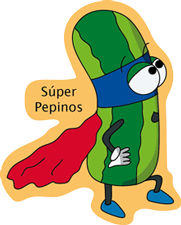
\includegraphics[scale=0.36]{../img/ttsuper}};
\end{tikzpicture}
\fi

\end{Slide}


\begin{Slide}{Abstrakta och konkreta medlemmar}
\vspace{-0.5em}\scalainputlisting[numbers=left,numberstyle=,basicstyle=\fontsize{6}{7}\ttfamily\selectfont]{../compendium/examples/workspace/w07-inherit/src/vego1.scala}
\end{Slide}


\begin{Slide}{Undvika kodduplicering med hjälp av arv}
\scalainputlisting[numbers=left,numberstyle=,basicstyle=\fontsize{6}{7.3}\ttfamily\selectfont]{../compendium/examples/workspace/w07-inherit/src/vego2.scala}
\end{Slide}




\begin{Slide}{Varför kan kodduplicering orsaka problem?}
\begin{itemize}
\item Mer att skriva (inte jättestort problem)
\pause
\item Fler kodrader att läsa och förstå
\pause
\item Fler kodrader som påverkas vid tillägg
\pause

\item Fler kodrader att underhålla: 
\begin{itemize}
\item Om man rättar en bug på ett ställe måste man komma ihåg att göra \Alert{exakt samma ändring} på alla de ställen där kodduplicering förekommer $\rightarrow$ \Alert{risk för nya buggar}
\end{itemize}	

\pause

\item Principen på engelska: \code{ DRY == "Don't Repeat Yourself!"}

\pause

\item {Men det kan finnas tillfällen när kodduplicering faktiskt är att föredra: t.ex. om man vill att olika delar av koden ska vara helt oberoende av varandra.}
\end{itemize}	
\end{Slide}




\begin{Slide}{Överskuggning}
\vspace{-0.5em}\scalainputlisting[numbers=left,numberstyle=,basicstyle=\fontsize{6}{7.3}\ttfamily\selectfont]{../compendium/examples/workspace/w07-inherit/src/vego3.scala}
\end{Slide}

\begin{Slide}{En final medlem kan ej överskuggas}
\vspace{-0.5em}\scalainputlisting[numbers=left,numberstyle=,basicstyle=\fontsize{6}{7.3}\ttfamily\selectfont]{../compendium/examples/workspace/w07-inherit/src/vego4.scala}
\end{Slide}


\begin{Slide}{Protected ger synlighet begränsad till subtyper}
\begin{REPL}
scala> trait Super { 
         private val minHemlis = 42
         protected val vårHemlis = 42
       }

scala> class Sub extends Super { def avslöjad = minHemlis } 
error: not found: value minHemlis

scala> class Sub extends Super { def avslöjad = vårHemlis } 
       
scala> val s = new Sub
s: Sub = Sub@2eee9593

scala> s.avslöjad
res0: Int = 42

scala> s.minHemlis
error: value minHemlis is not a member of Sub       

scala> s.vårHemlis
error: Access to protected value vårHemlis not permitted 
\end{REPL}
\end{Slide}


\begin{Slide}{Filnamnsregler och -konventioner}
\begin{itemize}
\item Java
\begin{itemize}
\item I Java får man bara ha \Alert{en enda} publik klass per kodfil.
\item I Java måste kodfilen ha \Alert{samma namn} som den publika klassen, t.ex. \code{KlassensNamn.java}
\end{itemize}
\item Scala
\begin{itemize}
\item I Scala får man ha \Emph{många} klasser/traits/singelobjekt i samma kodfil.
\item I Scala får man döpa kodfilerna \Emph{oberoende} av deras innehåll. \pause Dessa \Emph{konventioner} används:
\begin{itemize}
\item Om en kodfil bara innehåller \Emph{en enda} klass/trait/singelobjekt ge filen samma namn som innehållet, t.ex. \code{KlassensNamn.scala} 
\item Om en kodfil innehåller \Emph{flera} saker, döp filen till något som återspeglar hela innehållet och använd \Emph{liten begynnelsebokstav}, t.ex. \code{drawing.scala} eller \code{bastypensNamn.scala} 
\end{itemize}


\end{itemize}

\end{itemize}
\end{Slide}


\begin{Slide}{Klasser, arv och klassparametrar}\SlideFontTiny
Klasser kan ärva klasser. Om superklassen har klassparametrar måste primärkonstruktor ges argument efter \code{extends}.

\scalainputlisting[numbers=left,numberstyle=,basicstyle=\fontsize{6.4}{7.7}\ttfamily\selectfont]{../compendium/examples/workspace/w07-inherit/src/personExample1.scala}

\end{Slide}


\begin{Slide}{Statisk och dynamisk typ}\SlideFontSmall
\begin{Code}
    var p: Person = new Forskare("Robin Smith", "Lund", "Professor Dr")
\end{Code}
\begin{itemize}
\item Den \Emph{statiska typen} för \code{p} är \code{Person} vilket gör att vi sedan kan låta \code{p} referera till andra instanser som är av typen Person.
\begin{Code}
p = new Student("Kim Robinson", "Lund", "Data")
\end{Code}

\pause

\item Med ''statisk typ'' menas den typinformation som kompilatorn känner till vid kompileringstid.

\pause
\item Den \Emph{dynamiska typen}, även kallad \Emph{körtidstypen}, som gäller under körning är här mer specifik och mångfaceterad: \code{p} är efter tilldelning nu Student, Person och Akademiker (men inte Examinerad). 

\pause

\item Man kan undersöka om den dynamiska typen för \code{p} är \code{EnVissTyp} med  \code{p.isInstanceOf[EnVissTyp]}

\pause

\item Man kan säga åt kompilatorn: \emph{''jag garanterar att p är av typen \code{EnVissTyp} så du kan omforma den till \code{EnVissTyp}''} med  \code{p.asInstanceOf[EnVissTyp]} \\ \pause (detta är inte så vanligt i normal Scala-kod) 
\end{itemize}
\end{Slide}




\begin{Slide}{Inmixning}\SlideFontTiny
Man kan ärva flera traits. Detta kallas inmixning \Eng{mix-in} och görs med \code{with}.
\scalainputlisting[numbers=left,numberstyle=,basicstyle=\fontsize{6.4}{7.7}\ttfamily\selectfont]{../compendium/examples/workspace/w07-inherit/src/personExample2.scala}
\end{Slide}



\begin{Slide}{\texttt{isInstanceOf} och \texttt{asInstanceOf}}\SlideFontTiny
Testa körtidstyp med \code{isInstanceOf[Typ]}. Lova kompilatorn (och ta själv ansvar för) att det är en viss körtidstyp med \code{asInstanceOf[Typ]}. OBS! Använd hellre \code{match}.
\scalainputlisting[basicstyle=\small\SlideFontSize{6.2}{7.6}\ttfamily\selectfont]{../compendium/examples/workspace/w07-inherit/src/personExample3.scala}
\end{Slide}



\begin{Slide}{Polymorfism och dynamisk bindning}\SlideFontTiny
\begin{Code}[basicstyle=\SlideFontSize{6.2}{7.5}\ttfamily\selectfont]
trait Robot { def work(): Unit }

case class CleaningBot(name: String) extends Robot {
  override def work(): Unit = println(" Städa Städa")
}

case class TalkingBot(name: String) extends Robot {
  override def work(): Unit = println(" Prata Prata")
}
\end{Code}
\Emph{Polymorfism} betyder ''många former''. Referenserna r och bot nedan kan ha olika ''former'', d.v.s de kan referera till olika sorters robotar. \\ \Emph{Dynamisk bindning} innebär att körtidstypen avgör vilken metod som körs.
\begin{REPL}[numbers=left, basicstyle=\color{white}\SlideFontSize{6.2}{7.5}\ttfamily\selectfont]
scala> def robotDoWork(bot: Robot) = { print(bot); bot.work }

scala> var r: Robot = new CleaningBot("Wall-E")

scala> robotDoWork(r)
CleaningBot(Wall-E) Städa Städa

scala> r = new TalkingBot("C3PO")

scala> robotDoWork(r)
TalkingBot(C3PO) Prata Prata
\end{REPL}
\end{Slide}

\Subsection{Uppräknade värden}


\begin{Slide}{Uppräknade värden med heltal}\SlideFontSmall
Vi kan använda heltalskonstanter för att representera olika färger.
\begin{Code}
object Färg {
  val Spader = 1
  val Hjärter = 2
  val Ruter = 3
  val Klöver = 4
}
\end{Code}
\begin{Code}[language=,keywords={case,class}]
case class Kort(färg: Int, valör: Int)
\end{Code}

Vi kan nu använda våra uppräknade färgvärden så här:
\begin{REPLnonum}
scala> import Färg._
scala> Kort(Ruter, 7)
\end{REPLnonum}
\pause Men kompilatorn \Alert{kan inte hindra} denna bugg:
\begin{REPLnonum}
scala> Kort(42, 7)
\end{REPLnonum}

\end{Slide}


\begin{Slide}{Uppräknade värden med case-objekt}\SlideFontSmall
Vi kan använda case-objekt för att representera olika färger.
\begin{Code}[language=,keywords={sealed,trait,object,case,class,extends}]
sealed trait Färg
case object Spader  extends Färg
case object Hjärter extends Färg
case object Ruter   extends Färg
case object Klöver  extends Färg

case class Kort(färg: Färg, valör: Int)
\end{Code}

Vi kan nu använda våra uppräknade färgvärden så här:
\begin{REPL}
scala> Kort(Ruter, 7)

scala> Kort(Spader, 1)
\end{REPL}
\begin{itemize}
\item Kompilatorn \Emph{garanterar} att vi bara använder exakt dessa färger.

\item Nyckelordet \code{sealed} förhindrar fler subtyper förutom de som finns här.

\item \code{case} före \code{object} ger en najs \code{toString} och möjliggör matchning \\
(mer om matchning i w10).

\end{itemize}

\end{Slide}

\begin{Slide}{Uppräknade värden i samling}\SlideFontSmall
Vi kan placera case-objekten i en samling som kan användas i loopar. \\ Ett lämpligt ställe för en sådan samling är i kompanjonsobjektet till \code{Färg}.
\begin{Code}
sealed trait Färg
object Färg { 
  val values = Vector(Spader, Hjärter, Ruter, Klöver)
}
case object Spader extends Färg
case object Hjärter extends Färg
case object Ruter extends Färg
case object Klöver extends Färg
\end{Code}

\begin{REPL}
scala> val allaEss = for (f <- Färg.values) yield Kort(f, 1)
\end{REPL}
\end{Slide}


\begin{Slide}{Uppräknade värden med heltalsomvandling}\SlideFontSmall
Med en \code{sealed abstract class} och ett heltalsattrribut \code{toInt} som klassparameter kan vi erbjuda omvandling till heltal.
\begin{Code}
sealed abstract class Färg(final val toInt: Int)
object Färg { 
  val values = Vector(Spader, Hjärter, Ruter, Klöver)
}
case object Spader  extends Färg(0)
case object Hjärter extends Färg(1)
case object Ruter   extends Färg(2)
case object Klöver  extends Färg(3)
\end{Code}

\begin{REPL}
scala> Kort(Ruter, 1).färg.toInt
res0: Int = 2
\end{REPL}
Nyckelordet \code{abstract} förhindrar instansiering av \code{Färg}. \\
Nyckelordet \code{final} förhindrar överskuggning av attributet \code{toInt}. \\
Nyckelordet \code{sealed} förhindrar vidare subtypning av \code{Färg}.
\end{Slide}



\Subsection{Exempel: Shape}


\begin{Slide}{Exempel: shapes1.scala}
Typisk Scala-kod: En trait som bastyp åt flera case-klasser.
\scalainputlisting[numbers=left,numberstyle=,basicstyle=\fontsize{6.4}{7.7}\ttfamily\selectfont]{../compendium/examples/workspace/w07-inherit/src/shapes1.scala}
\end{Slide}

\begin{Slide}{Exempel: shapesTest1.scala}
Test av konkreta subklasser till bastypen \code{Shape}.
\scalainputlisting[numbers=left,numberstyle=,basicstyle=\fontsize{6.4}{7.7}\ttfamily\selectfont]{../compendium/examples/workspace/w07-inherit/src/shapesTest1.scala}

\begin{REPL}
Rectangle((100.0,100.0),(75.0,120.0))
Rectangle((141.0,183.0),(75.0,120.0))
Triangle((0.0,0.0),(4.0,0.0),(4.0,3.0))
Triangle((1.0,1.0),(4.0,0.0),(4.0,3.0))
Triangle((0.0,0.0),(4.0,0.0),(4.0,3.0))
\end{REPL}
\end{Slide}


\begin{Slide}{Exempel: draw.scala}
Två traits som kan användas för att ''koppla ihop'' kod och minimera ändringar av befintlig kod:
\scalainputlisting[numbers=left,numberstyle=,basicstyle=\fontsize{7}{9}\ttfamily\selectfont]{../compendium/examples/workspace/w07-inherit/src/draw.scala}

\pause
\setlength{\leftmargini}{0pt}
\begin{itemize}\SlideFontSmall
\item  Traits som använda för att abstrahera implementation och möjliggöra uppfyllandet av ett slags ''kontrakt'' om vad som ska finnas kallas \Emph{gränssnitt} \Eng{interface} och är grunden för skapandet av ett flexibelt api. 

\item Implementationen av de delar vi vill kunna ändra senare placeras i subtyper som inte används direkt av klientkoden. 

\item Vi visar bara information om vad som erbjuds men inte hur det ser ut ''inuti''.

\end{itemize}
\end{Slide}

\begin{Slide}{Exempel: shapes2.scala}\SlideFontTiny
Genom att \Emph{mixa in} vår \code{trait CanDraw} kan en rektangel nu även ritas ut:

\scalainputlisting[numbers=left,numberstyle=,basicstyle=\fontsize{6.5}{7.8}\ttfamily\selectfont]{../compendium/examples/workspace/w07-inherit/src/shapes2.scala}

\pause
\vspace{-0.5em}Notera: ingen ändring i \code {Shape}! Vi behöver nu bara ett \Emph{\code{DrawingWindow}}...
\end{Slide}


\begin{Slide}{Exempel: SimpleDrawingWindow.scala}\SlideFontTiny
\vspace{-0.35em}
Vi skapar en ny klass som ärver \code{SimpleWindow}, som \Alert{dessutom} även \Emph{är ett} \code{DrawingWindow}, tack vare \Emph{inmixning} med nyckelordet \code{with}.\\
Observera att vi måste skicka vidare klassparametrarna till superklassens konstruktor. 

\scalainputlisting[numbers=left,numberstyle=,basicstyle=\fontsize{6.4}{7.7}\ttfamily\selectfont]{../compendium/examples/workspace/w07-inherit/src/SimpleDrawingWindow.scala}

\pause
\vspace{-0.35em}
\scalainputlisting[numbers=left,numberstyle=,basicstyle=\fontsize{6.4}{7.7}\ttfamily\selectfont]{../compendium/examples/workspace/w07-inherit/src/shapesTest2.scala}
\end{Slide}


%\begin{Slide}{Exempel: Robot}
%\begin{center}
%\newcommand{\TextBox}[1]{\raisebox{0pt}[1em][0.5em]{#1}}
%\begin{tikzpicture}[inner sep=0.5em]
%\node [umlclass, rectangle split parts = 2, xshift=0cm] (AbstractRobot)  {
%            \textit{\textbf{\centerline{\TextBox{AbstractRobot}}}}
%            \nodepart[]{second}\TextBox{work(): void}
%        };
%        
%\node [umlclass, rectangle split parts = 2]  at (2cm,-3cm) (MuteRobot) {
%            \textbf{\centerline{\TextBox{MuteRobot}}}
%            \nodepart[]{second} \TextBox{~}
%        };  
%                
%\node [umlclass, rectangle split parts = 2] at (-2cm,-3cm) (TalkingRobot)  {
%            \textbf{\centerline{\TextBox{TalkingRobot}}}
%            \nodepart[]{second} \TextBox{talk(): void}
%        };        
%\draw[umlarrow] (TalkingRobot.north) -- ++(0,0.5) -| (AbstractRobot.south);    
%\draw[umlarrow] (MuteRobot.north) -- ++(0,0.5) -| (AbstractRobot.south);            
%\end{tikzpicture}
%\end{center}
%\end{Slide}






\begin{Slide}{Attribut och metoder i UML-diagram}
\begin{center}
\begin{tikzpicture}
\node (Class) [umlclass, rectangle split parts = 3, xshift = -2cm, yshift=-1.5cm, text width = 4.2cm, scale=0.8]  {
            \textbf{\centerline{Name}}
            \nodepart[]{second}attr1: Type \newline attr2: Type
            \nodepart[]{third}method1(a: Type): Type \newline  method2(b: Type): Type
       };
\node (explain1)[above of = Class, yshift=1cm, text width=4.9cm]{En klass i ett \Emph{UML}-diagram kan ha 3 delar:};
\node (explain2)[below of = Class, yshift=-1cm]{Ibland utelämnar man typerna.};



\node [umlclass, rectangle split parts = 3]  at (4,0) (Robot) {
            \textbf{\centerline{Robot}}
            \nodepart[]{second}name: String
            \nodepart[]{third}work(): Unit
       };
\node [umlclass, rectangle split parts = 3]  at (4, -3) (TalkingRobot)  {
            \textbf{\centerline{TalkingRobot}}
            \nodepart[]{second} phrase: String           
            \nodepart[]{third}speak(): Unit
        };        
\draw[umlarrow] (TalkingRobot.north) -- ++(0,0.8) -| (Robot.south);        
\end{tikzpicture}
\end{center}
\hskip2em\href{https://en.wikipedia.org/wiki/Class_diagram}{\SlideFontTiny en.wikipedia.org/wiki/Class\_diagram}
\end{Slide}




